\section{Rewriting RBAs in full matrix form}

\paragraph{Composition vector for macromolecules} In the following, each macromolocule is described by its \textbf{composition vector}. It is a column vector containing the metabolites necessary to build it, with a \textbf{minus} sign for metabolites consumed and a \textbf{plus} sign for byproducts generated.

\paragraph{Metabolism constraint} The metabolism constraint $(C_1)$ can be rewritten

\[
\overbrace
{
\underbracket{S\nu}_{\parbox{2cm}{\scriptsize metabolic flux generated by metabolism}} 
+
\underbracket{\mu [C_E,C_R,C_C] [E;R;C]}_{\parbox{3cm}{\scriptsize precursors used/byproducts generated by producing new molecules}}
}^{\text{\normalsize `Variable' terms}}
=
\overbrace
{
\underbracket{-\mu [C_{G},C_{X_c}] [P_G;X_c]}_{\parbox{3cm}{\scriptsize precursors used/byproducts generated by producing new molecules}}
}^{\text{\normalsize Constant terms}} \\
\]
\[
-\diag{k_E} E \leq \nu \leq \diag{k_E} E
\]

where $C_{i}$ are composition matrices as defined above.

Written this way, it actually does not matter to which group a metabolite belongs. Its group is only dictated by the structures of the composition matrices. Based on this constraint only it does not make sense to create metabolic groups \emph{in the program}.

In full matrix form, the above equations become
\[
\left\{
\begin{array}{ccc}
  [S, \mu C_E, \mu C_R, \mu C_C][\nu;E;R;C]
  & = & - [\mu C_G,\mu C_{X_c}][P_G;X_c] \\
  \left[
    \begin{array}{cccc}
      I, & -\diag{k_E}, & 0, & 0 \\
      -I, & -\diag{k_E}, & 0, & 0
    \end{array}
    \right]
       [\nu; E;R;C] &\leq & 0
\end{array}
\right.
\]

The most important here is the composition matrix. In the data, the user gives the list of metabolites used for synthesis and the list of byproducts. The program then has to figure out how to reorder terms to build the matrix.

\paragraph{Ribosome/chaperone constraints} We can rewrite the ribosome constraint as follows:
\[
k_TR = \mu [PC^R_E,PC^R_R,PC^R_C] [E;R;C] + \mu PC^R_GP_G
\]
where $PC^R$ is the Processing Cost of a molecule and $k_T$ the capacity of a ribosome (\textit{e.g.} the capacity of a ribosome is the number of aas it can process and the processing cost is the number of amino acids of a protein).
In full form:
\[
[0,\mu PC^R_E,k_T+\mu PC^R_R,\mu PC^R_C] [\nu;E;R;C] = [-\mu PC^R_G,0][P_G;X_c]
\]

The same applies for folding by chaperones. 

These additionnal constraints have the form
\[
a [\nu; E; R; C] = b_0 + b_1 [P_G;X_c]
\]
this means they can be appended to $C_1$ by \textbf{simple line concatenation}.

\paragraph{RNA degradation/replication} In this type of constraints, we simply add new fluxes of metabolites. These fluxes are simply added up on the right hand side of $(C_1)$
\[
\begin{array}{rcl}
...  & = & -\mu[C_G,C_{X_c}][P_G;X_c] - \mu^{d}C_{process}X_{process} \\
 & =  & -[\mu C_G, \mu C_{X_c},\mu^d C_{process}][P_G;X_c;X_{process}]
\end{array}
\]
where $d = 0$ when the target flux is an abolute flux and $d=1$ when it compensates dilution.

\paragraph{Density constraints} The density constraint writes
\[
[0,W_E,W_R,W_C] [\nu;E;R;C] \leq \overline{D} - [W_G,W_c][P_G;X_c]
\]
where $W$ is the weight of each molecule.
In general, these constraints can be expected to be of the form
\[
a [\nu; E; R; C] \leq b_0 + b_1 [P_G;X_c]
\]

\paragraph{Maintenance ATP constraint (flux constraints)} It is defined as
\[
\mathbf{1}_{\nu_{constraint}} [\nu; E; R; C] = b
\]
where $\mathbf{1}_{\nu_{constraint}}$ is an indicator matrix selecting the reaction associated with the production of maintenance ATP/flagella fuel. Generally this means a specific reaction has to be added in $S$. Another way to handle these constraints is to include them in the lower/upper bounds of the optimization problem.

\paragraph{Summary}

\[
\begin{array}{ccll}
  [S, \mu C_E, \mu C_R, \mu C_C] & [\nu;E;R;C] = & 
  - \sum \mu^{d_i}C_i X_i & \textrm{(Base metabolism}\\
  & & & \textrm{and process production)} \\
  a & [\nu; E; R; C] = & b_0 + b_1 [\{X_i\}] & \textrm{(Process capacity)}\\
  \mathbf{1}_{\nu_{constraint}} & [\nu; E; R; C] = & b & \textrm{(Flux constraints)} \\
  \left[
    \begin{array}{cccc}
      I, & -\diag{k_E}, & 0, & 0 \\
      -I, & -\diag{k_E}, & 0, & 0
    \end{array}
    \right] & [\nu; E;R;C] \leq & 0 & \textrm{(Enzymatic fluxes)}\\
  a & [\nu; E; R; C] \leq & b_0 + b_1 [\{X_i\}] & \textrm{(Density constraints)} \\
\end{array}	
\]

A more graphic representation of the matrix is provide in \reffigt{fig:new_matrices_rba}.

\begin{figure}[ht]
  \centering
  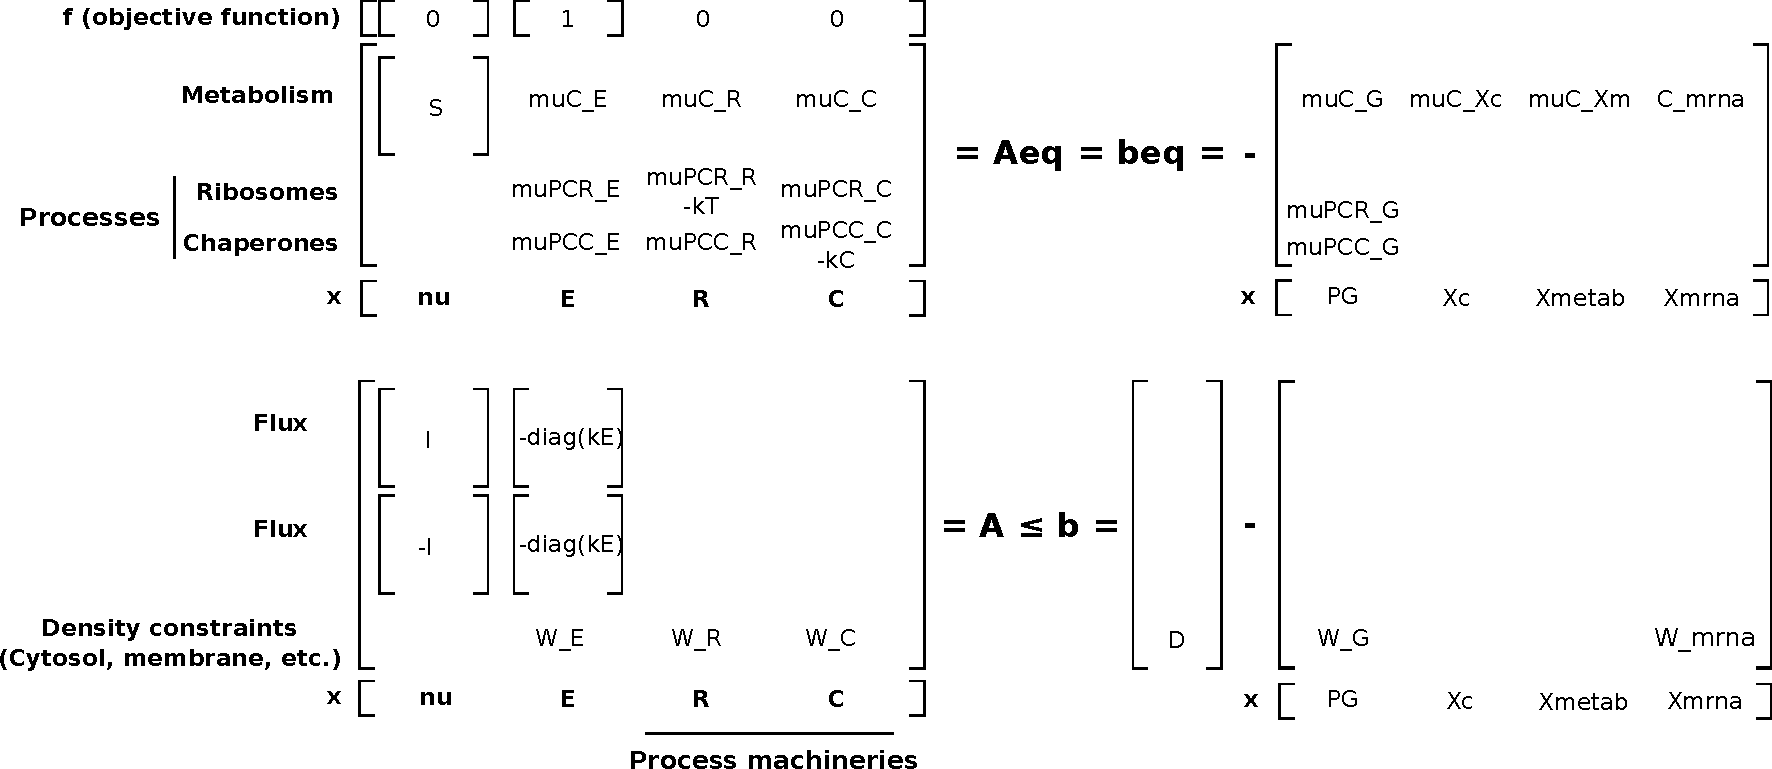
\includegraphics[width=\linewidth]{new_matrices_RBA}
  \caption{Structure of matrices. Note that the left hand side and the right hand side have a similar structure (except for the $\nu$ submatrix). Each column represents a set of molecules: on the right hand side, the production flux of the set has to be determined, on the left hand side it is already given \textit{a priori}.}
  \label{fig:new_matrices_rba}
\end{figure}
